\documentclass[11pt]{article}
\usepackage[margin=.85in]{geometry}
\usepackage{amsmath,amssymb,booktabs,enumitem,graphicx,hyperref,microtype}
\usepackage{xcolor}
\graphicspath{{../shared/results/paper2_9_look_ahead_back/}}
\hypersetup{colorlinks=true,linkcolor=blue!55!black,citecolor=blue!55!black,urlcolor=blue!55!black}
\newcommand{\pra}{\textsc{PRA}}
\newcommand{\paperii}{Paper~2.8}
\title{Temporal Query Windows for Progressive Retrieval Attention\\
\large A Negative Retrieval Result and a Slower Routing Clock}
\author{Jorge Sim\~ao\\EInnovator R\&D -- Center for the Sciences of Computation, Cognition, and Complexity}
\date{August 2026}

\begin{document}
\maketitle

\begin{abstract}
Progressive Retrieval Attention (\pra) separates memory discovery from native-key/value materialization. Prior work improved the memory side of discovery by replacing a mean gist with learned key landmarks. This paper asks whether the query side should likewise aggregate several adjacent hidden states instead of routing from one state. We replay tokenwise, pre-RoPE queries from a frozen Qwen3-0.6B backbone over identity-disjoint HotpotQA, QASPER, 2WikiMultiHopQA, and MuSiQue cohorts. Five frozen Paper~2.8 compressors are evaluated with causal windows, four reducers, delayed commitment, an analysis-only known-future condition, sparse routing clocks, and bounded lexical fusion. Exact replay parity is established before new comparisons. Validation chooses a two-token window on every dataset, yet its held-out recall change relative to the same reducer at one token is $-0.0223$, $-0.0081$, $-0.0098$, and $+0.0011$, respectively; every paired 95\% confidence interval crosses zero. Known-future gains at a four-token anchor are also small, from $-0.0087$ to $+0.0102$. These results close the prefill and predictive-look-ahead branches under the predeclared gate. The useful result is computational: routing every four tokens reduces calls to $0.30$--$0.36$ per token with at most $0.0107$ absolute recall loss. Temporal pooling therefore does not repair retrieval in this setting, but a slower routing clock appears viable. The positive advantage of learned memory landmarks on QASPER and 2Wiki remains intact and should not be attributed to temporal aggregation.
\end{abstract}

\section{Introduction}
Autoregressive transformers generate one token at a time, but a retrieval decision need not be recomputed at the same rate. A name may become discriminative only after its qualifier, a relation may span several tokens, and a question may expose its target gradually. These facts motivate an apparently simple extension to \pra: route from a short temporal window of query states rather than the current state alone.

The extension is not automatically useful. A late hidden state already contains causal history, so explicit pooling can add little information while blurring a sharp query. Delaying a decision changes both the available evidence and the set of token positions being scored. Looking ahead during prompt prefill is technically possible, but it is not evidence that a causal decoder can obtain the same signal during generation. This study therefore treats temporal routing as a controlled falsification problem rather than as a presumed improvement.

We integrate temporal queries with the learned native-key compressors from \paperii. The memory representatives, candidate chunks, materialization budget, frozen backbone, and validation/test identities remain fixed. Only the query construction and routing schedule change. This gives a direct answer to the central question: does more temporal query context improve discovery once memory-side compression is already strong?

The contributions are:
\begin{enumerate}[leftmargin=*]
\item a tokenwise capture and replay path for pre-RoPE Qwen3 query states with exact inherited-selection parity;
\item a matched study spanning four natural datasets, five seeds, causal windows, late interaction, delayed commitment, known-future analysis, and routing stride;
\item an explicit $2\times2$ query-window by memory-compressor contrast that prevents memory-side gains from being misreported as temporal gains;
\item a negative quality result: no validation-selected temporal policy improves held-out evidence recall with a paired confidence interval above zero;
\item a positive systems result: a stride-four routing clock preserves recall within $0.011$ while using only $0.30$--$0.36$ router calls per token.
\end{enumerate}

\section{Relation to prior work}
Sparse and retrieval-augmented transformers reduce attention or context cost through fixed sparse patterns, external retrieval, recurrent memory, or cache selection \cite{beltagy2020longformer,zaheer2020bigbird,lewis2020rag,borgeaud2022retro,rae2020compressive,li2024snapkv}. Late-interaction retrievers preserve multiple token-level comparisons instead of collapsing both sides to single vectors \cite{khattab2020colbert}. Transformer-XL and related recurrent systems carry prior hidden state forward, while adaptive computation changes how often or how deeply a model updates \cite{dai2019transformerxl,graves2016adaptive}. Our question is narrower: with a frozen decoder and fixed native-K/V memory candidates, does a short query-side temporal window improve which chunks are selected?

Within the \pra series, Paper~2.5 studies iterative associative traversal, Paper~2.6 combines semantic and token-native channels, and Paper~2.7 studies graph-derived query facets. \paperii{} studies memory-side QK compression and supplies the frozen rank-16 and rank-8/centroid-8 compressors used here. Paper~2.9 changes the temporal extent of the semantic query. It does not alter native-K/V materialization, train the language model, or claim end-to-end generation gains.

The scope distinction matters. Explicit strings such as URIs, API paths, exact aliases, headings, or symbols remain natural targets for indexed lexical routing. Temporal hidden-state pooling instead targets natural-language queries whose discriminating evidence unfolds over adjacent tokens.

\section{Temporal routing}
\subsection{Captured query states}
At decoder layer $\ell$ and token position $t$, let $q_{t}^{\ell}\in\mathbb{R}^{d_h}$ denote the pre-RoPE query vector replayed from the frozen layer input, its native input normalization, and the layer's query projection. Earlier decoder blocks execute normally. The capture wrapper observes the target layer without modifying its output. Attention masks, question spans, token positions, identity, split, and source provenance are stored with each trace.

We capture the embedding projection diagnostic and layers $8$, $18$, and $27$, using layer $27$ for the main study. Captured tensors are FP16 on disk and promoted for scoring. Against online replay, the maximum absolute FP16 deviation is $0.015625$ and the mean deviation is $6.52\times10^{-4}$. More importantly, inherited chunk selections and recall are reproduced exactly before temporal policies are evaluated.

\subsection{Causal windows and reducers}
For a causal history length $B$, define
\begin{equation}
Q_{t,B}^{\ell}=\{q_{t-B+1}^{\ell},\ldots,q_t^{\ell}\},
\end{equation}
clipped at the question boundary. We test $B\in\{1,2,4,8,16\}$. Four parameter-free reducers isolate plausible temporal mechanisms:
\begin{align}
r_{\mathrm{mean}}(Q)&=|Q|^{-1}\sum_{q\in Q}q,\\
r_{\mathrm{recency}}(Q)&=\frac{\sum_{j=1}^{|Q|}\exp(\alpha j)q_j}{\sum_{j=1}^{|Q|}\exp(\alpha j)},\\
s_{\mathrm{late\mbox{-}max}}(Q,k)&=\max_{q\in Q}\langle q,k\rangle,\\
s_{\mathrm{late\mbox{-}top}}(Q,k)&=K^{-1}\sum_{z\in\operatorname{TopK}\{\langle q,k\rangle:q\in Q\}}z.
\end{align}
Mean and recency produce one query vector. Late-max and late-top-mean retain token-to-landmark interactions until scoring. The current-state baseline is $B=1$; because it ignores extra history, it is excluded from nontrivial temporal model selection.

\subsection{Memory representatives and the factorial contrast}
The memory side uses the frozen conditions inherited from \paperii: a native mean gist, a rank-16 learned landmark selector, and a rank-8 selector with eight centroids. For query condition $Q\in\{\text{one-state},\text{window}\}$ and memory condition $M\in\{\text{mean},\text{learned}\}$, let $R(Q,M)$ be evidence recall at four selected chunks. The interaction is
\begin{equation}
\Delta_{Q\times M}=R(Q_w,M_l)-R(Q_1,M_l)-R(Q_w,M_m)+R(Q_1,M_m).
\end{equation}
This difference-in-differences asks whether temporal context specifically unlocks a learned memory representation. A positive memory-compressor main effect is not, by itself, support for temporal routing.

\subsection{Delay, known future, and routing stride}
At matched anchor positions, the immediate condition routes from observed history ending at $t$. Fixed delay $D$ waits until $t+D$, after which those tokens are ordinary causal history. The known-future condition exposes the same future span to the anchor query and is analysis-only. It estimates headroom; it is not described as a deployable causal method.

Routing stride $s\in\{1,2,4,8\}$ recomputes every $s$ tokens and reuses the selected chunk set between calls. We report calls per token and recall relative to stride one. This tests whether semantic discovery can operate on a slower clock even when wider temporal pooling is unhelpful.

\section{Experimental protocol}
\subsection{Data and frozen components}
The study uses the inherited identity-disjoint cohorts from HotpotQA \cite{yang2018hotpotqa}, QASPER \cite{dasigi2021qasper}, 2WikiMultiHopQA \cite{ho2020twowiki}, and MuSiQue \cite{trivedi2022musique}. The captured set contains 288 identities: 8 validation and 16 test identities each for HotpotQA and QASPER, and 20 validation plus 100 test identities each for 2Wiki and MuSiQue. These cohort sizes support matched mechanistic comparisons, not broad benchmark claims.

The backbone is frozen Qwen3-0.6B revision \texttt{c1899de289a04d12100db370d81485cdf75e47ca} \cite{qwen2025qwen3}. Five frozen Paper~2.8 checkpoints are score-ensembled. No temporal module, backbone weight, memory compressor, or language-model head is trained here. Validation selects each dataset policy; test identities are opened once for the reported effect.

\subsection{Budgets and metrics}
All primary conditions select four unique memory chunks. Candidate memories, evidence annotations, and chunk budgets are inherited. The primary metric is identity-level evidence recall at four chunks. We also record complete-evidence recovery, reciprocal rank, score entropy and margin, candidate count, selected-set churn, router calls per token, component latency, and index storage. Confidence intervals are paired nonparametric bootstraps over identities, never over overlapping token windows.

The bounded hybrid control combines semantic scores with exact-token/BM25 evidence. Lexical weight is selected on validation data. The predeclared temporal quality gate requires a validation-selected $B>1$ condition whose paired 95\% interval is above zero on at least one natural dataset, with no absolute regression larger than $0.02$ on the other primary dataset. Known-future gain must exceed $0.02$ before a prefill sidecar or predictive future probe is justified.

\subsection{Reproducibility and parity}
The implementation separates capture, temporal replay, statistical summarization, and cost audit. Each phase writes a manifest and resumable stage cache. The cache is excluded from version control; final per-example tables, summaries, figures, and gate decisions are tracked.

Historical Paper~2.8 selections are reproduced exactly: 80/80 seed-level selections for HotpotQA and QASPER and 100/100 for 2Wiki and MuSiQue. Historical recalls are likewise exact: $0.12104$, $0.25422$, $0.19028$, and $0.07093$. The original report averaged seed metrics on HotpotQA/QASPER but ensembled seed scores on 2Wiki/MuSiQue. To avoid a dataset-dependent estimator, all new Paper~2.9 comparisons use the five-seed score ensemble uniformly.

\section{Results}
\subsection{Temporal windows do not improve held-out retrieval}
Validation selected a two-token window on every dataset, although the reducer differed: mean on HotpotQA and late-top-mean on the other three. Table~\ref{tab:main} compares each selected policy with the same reducer and learned memory compressor at $B=1$. This is the clean temporal contrast. Three point estimates are negative; MuSiQue is effectively unchanged. Every confidence interval includes zero, so the temporal quality gate fails.

\begin{table}[t]
\centering
\caption{Held-out evidence recall at four chunks for the validation-selected temporal policy. $B=1$ uses the same reducer and memory compressor. Intervals are paired identity bootstraps.}
\label{tab:main}
\small
\begin{tabular}{lrrrr}
\toprule
Dataset & $B=1$ & Selected $B=2$ & $\Delta$ & 95\% CI \\
\midrule
HotpotQA & .1241 & .1018 & $-.0223$ & $[-.0692,.0179]$ \\
QASPER & .2846 & .2765 & $-.0081$ & $[-.0268,.0025]$ \\
2Wiki & .1903 & .1804 & $-.0098$ & $[-.0232,.0032]$ \\
MuSiQue & .0709 & .0721 & $+.0011$ & $[-.0060,.0085]$ \\
\bottomrule
\end{tabular}
\end{table}

\begin{figure}[t]
\centering
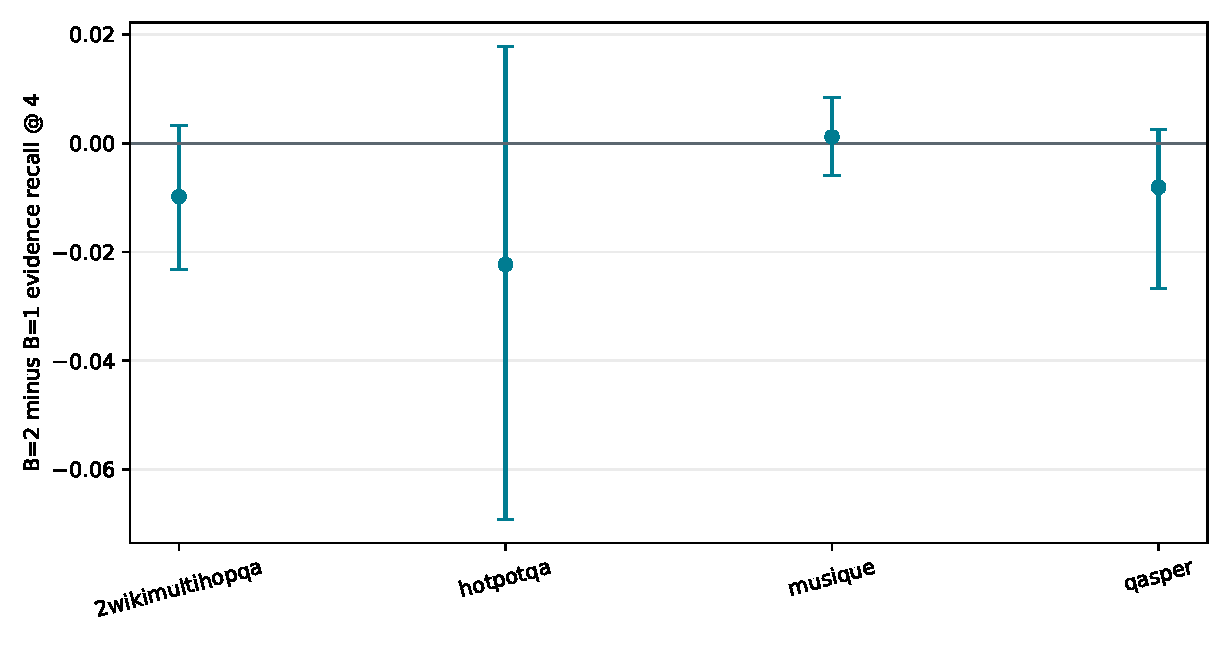
\includegraphics[width=.93\linewidth]{selected_temporal_effects.pdf}
\caption{Paired held-out effect of each validation-selected temporal policy relative to its same-reducer $B=1$ control. No interval excludes zero on the positive side.}
\label{fig:effects}
\end{figure}

The memory compressor remains consequential. Under the selected two-token policy, rank-16 recall is $.2765$ on QASPER versus $.1101$ for the native mean, a paired advantage of $.1663$ with 95\% CI $[.0340,.3204]$. On 2Wiki the corresponding values are $.1804$ and $.0914$, an advantage of $.0890$ with CI $[.0552,.1228]$. Rank-8/centroid-8 reaches $.2458$ and $.1743$. These are memory-side effects inherited from \paperii; Table~\ref{tab:interaction} shows that query widening does not amplify them.

\begin{table}[t]
\centering
\caption{Query-window by learned-memory interaction contrast. A positive value would indicate that temporal context specifically helps the learned compressor.}
\label{tab:interaction}
\begin{tabular}{lr}
\toprule Dataset & $\Delta_{Q\times M}$ \\
\midrule
HotpotQA & $-.0348$ \\
QASPER & $-.0206$ \\
2Wiki & $-.0036$ \\
MuSiQue & $+.0059$ \\
\bottomrule
\end{tabular}
\end{table}

Across layer diagnostics, later states are much stronger than the embedding projection but there is no universal best intermediate layer. For example, QASPER late-max $B=4$ recall is $.0292$ at the embedding probe, $.3413$ at layer 8, $.3541$ at layer 18, and $.3503$ at layer 27. This supports using contextual hidden queries, but not a claim that one layer or a wider temporal window is generally optimal.

\subsection{Known future exposes little actionable headroom}
Table~\ref{tab:delay} compares immediate, fixed-delay, and analysis-only known-future routing at the same four-token anchor. QASPER and 2Wiki show small positive future headroom; HotpotQA becomes worse and MuSiQue is nearly unchanged. No held-out gain exceeds the predeclared $.02$ threshold. At delay eight, QASPER's known-future gain rises to $.0174$, but only 12 identities retain enough matched positions.

\begin{table}[t]
\centering
\caption{Matched-anchor recall at $D=4$. Known future uses unavailable future states and is diagnostic only.}
\label{tab:delay}
\small
\begin{tabular}{lrrrr}
\toprule
Dataset & Immediate & Delayed & Known future & Future gain \\
\midrule
HotpotQA & .1043 & .0997 & .0955 & $-.0087$ \\
QASPER & .2868 & .2933 & .2971 & $+.0102$ \\
2Wiki & .1686 & .1713 & .1718 & $+.0033$ \\
MuSiQue & .0599 & .0604 & .0610 & $+.0011$ \\
\bottomrule
\end{tabular}
\end{table}

\begin{figure}[t]
\centering
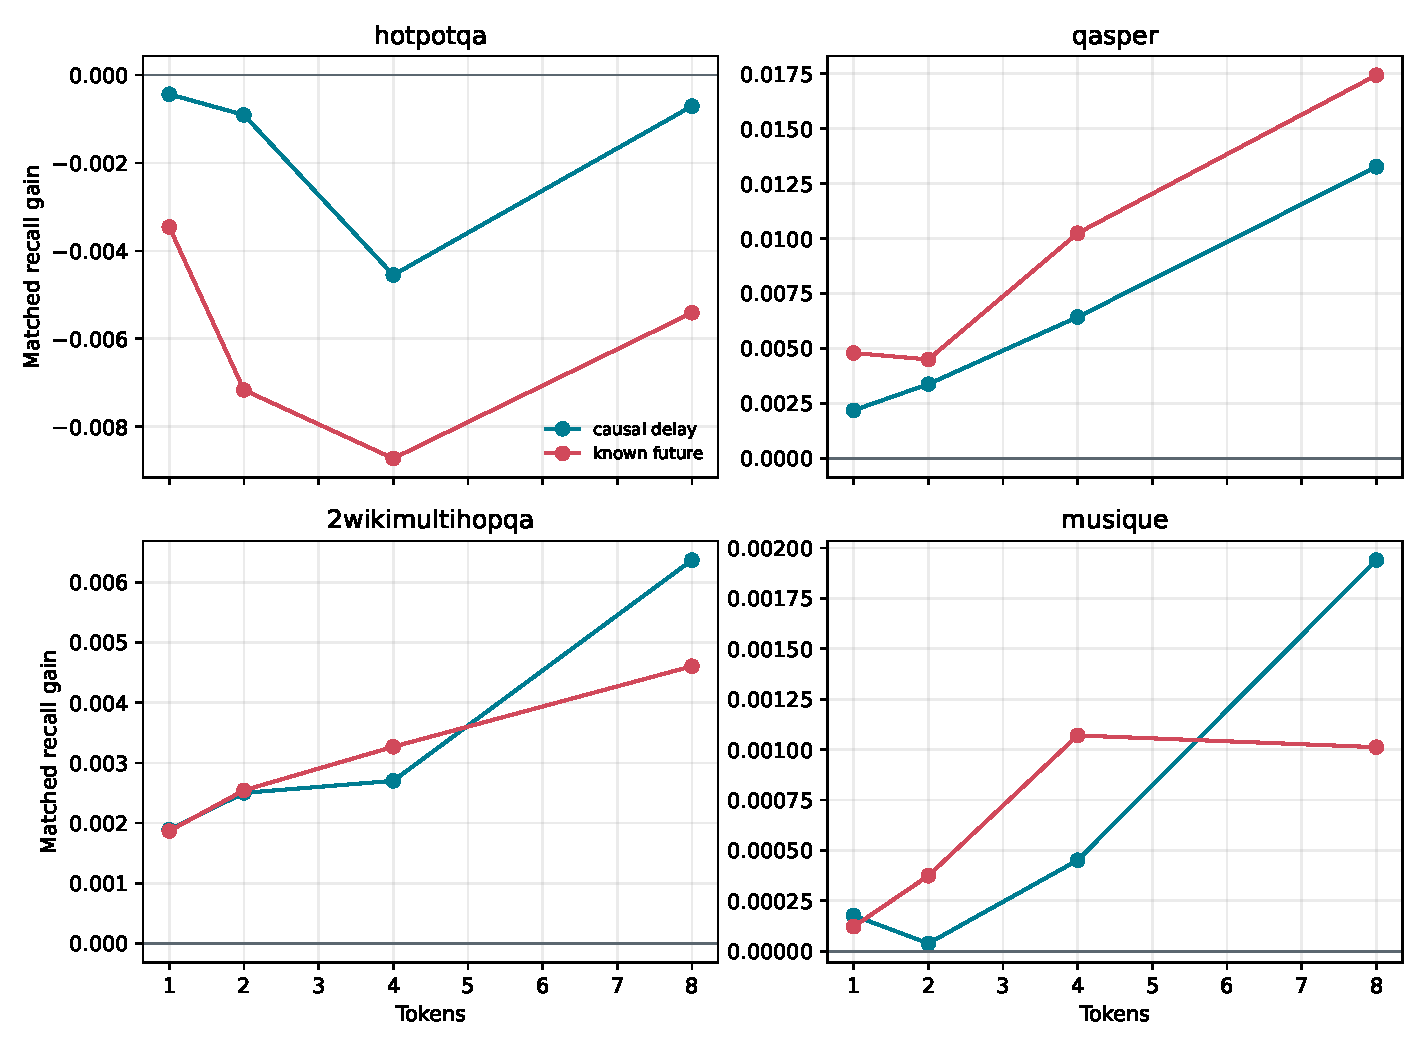
\includegraphics[width=.93\linewidth]{matched_delay_headroom.pdf}
\caption{Matched delayed-commitment and known-future effects. The future signal is too small and inconsistent to justify a learned predictive sidecar.}
\label{fig:delay}
\end{figure}

Because material known-future headroom is absent, the prefill-sidecar and predictive-future branches are closed rather than tuned until they succeed. Native-K/V consumption and answer generation are also not run: the predeclared retrieval gate was not met.

\subsection{Routing can run on a slower clock}
Temporal aggregation fails as a quality intervention, but decision reuse is robust. At stride four, calls fall to $.299$--$.361$ per token and recall changes by only $-.0012$, $-.0107$, $-.0050$, and $-.0023$ (Table~\ref{tab:stride}). This passes the efficiency gate of at most $.40$ calls per token and less than $.02$ absolute recall loss.

\begin{table}[t]
\centering
\caption{Stride-four routing frontier relative to recomputing every token.}
\label{tab:stride}
\begin{tabular}{lrrr}
\toprule
Dataset & Recall & Calls/token & $\Delta$ vs stride 1 \\
\midrule
HotpotQA & .0970 & .299 & $-.0012$ \\
QASPER & .2685 & .361 & $-.0107$ \\
2Wiki & .1680 & .323 & $-.0050$ \\
MuSiQue & .0568 & .302 & $-.0023$ \\
\bottomrule
\end{tabular}
\end{table}

\begin{figure}[t]
\centering
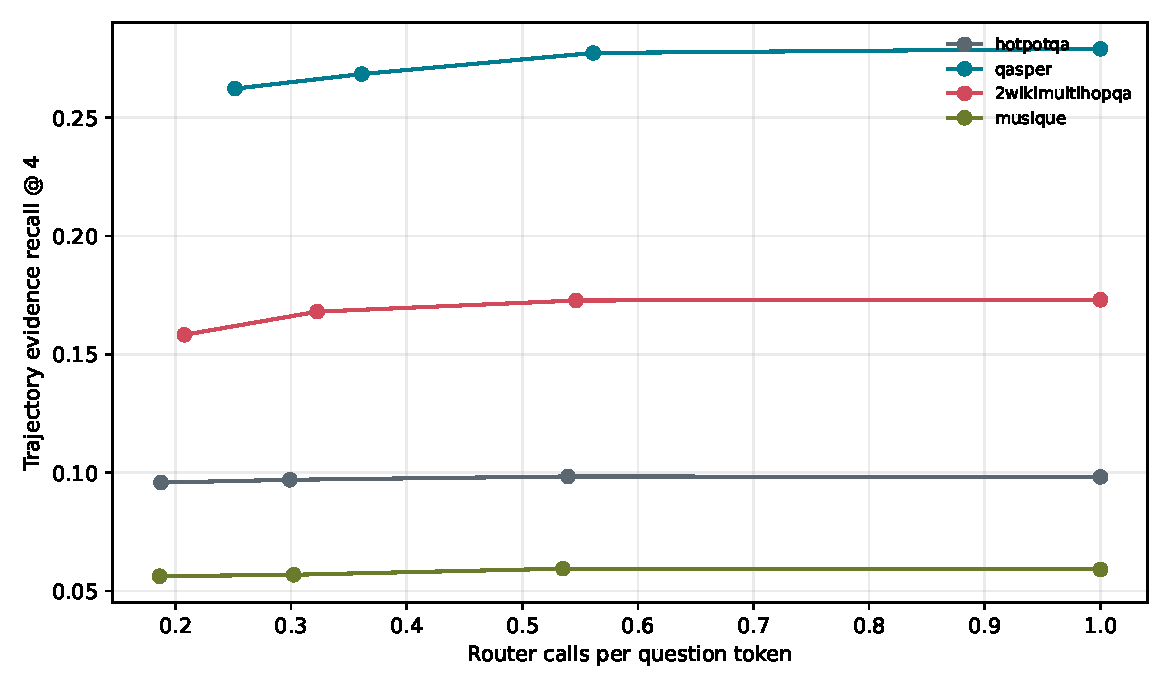
\includegraphics[width=.93\linewidth]{stride_quality_frontier.pdf}
\caption{Recall and router calls per token as the routing stride increases. Stride four is the predeclared operating point.}
\label{fig:stride}
\end{figure}

The CPU component audit measures cached five-seed ensemble routing only; it excludes the backbone and native-K/V transfer. A selected two-token call takes $1.42$ ms on HotpotQA, $2.51$ ms on QASPER, $1.73$ ms on 2Wiki, and $2.05$ ms on MuSiQue. Amortized at stride four these become $.35$, $.63$, $.43$, and $.51$ ms/token. Mean index construction ranges from $7.85$ to $22.53$ ms. These are implementation-component measurements on an Intel family-6 model-94 CPU, not end-to-end serving throughput claims.

\subsection{Lexical fusion and formal gates}
Validation selects zero lexical weight on all four datasets. Thus the bounded exact/BM25 fusion collapses to the semantic score and supplies no evidence of complementary channels in these cohorts. This result does not contradict Paper~2.6: exact and indexed channels remain appropriate for explicitly token-addressable memories, while these natural-language cohorts and frozen candidates do not expose the same geometry.

\begin{table}[t]
\centering
\caption{Predeclared gate outcomes.}
\label{tab:gates}
\small
\begin{tabular}{lll}
\toprule Gate & Status & Evidence \\
\midrule
I0/G0 & Pass & Exact inherited selection and recall parity \\
I1/G1 & Fail & No temporal CI lies above zero \\
I2/G4 & Fail & No positive query--memory interaction \\
G2 & Closed & Known-future gain stays below $.02$ \\
I3 & Pass & Stride 4: $\leq.40$ calls/token, loss $<.02$ \\
I4 & Fail & Validation selects lexical weight zero \\
G3/G5 & Not run & Sidecars gated by insufficient future headroom \\
I5/G6 & Not run & Retrieval gate does not justify generation \\
\bottomrule
\end{tabular}
\end{table}

\section{Why did temporal pooling fail?}
The most conservative explanation is representational redundancy. A late causal query state already summarizes preceding question tokens. Averaging neighboring states then repeats shared context and can attenuate the newest discriminative direction. Late interaction avoids literal averaging, but it also admits several partially formed queries; a distractor that matches any one token can win the maximum.

A second explanation is that query-side context was not the binding constraint. QASPER and 2Wiki improve substantially when the memory mean is replaced by learned landmarks, while widening the query does not add to that gain. Sparse evidence is therefore more often lost in memory compression than in the final query state for these conditions.

Third, the weak known-future result limits the value of more elaborate temporal machinery. If a non-causal diagnostic with the true future span adds at most about one recall point on the larger positive cases, a learned predictor has little room after approximation error and latency. The disciplined outcome is to close that branch, not to add capacity.

The stride result points in a different direction. Adjacent token decisions are similar enough that routing need not run every token, even though pooling their states does not improve ranking. Temporal redundancy is therefore useful for scheduling, not for query representation.

\section{Implementation sketch}
The core mechanism is deliberately small. A capture hook records frozen pre-RoPE query vectors and provenance. Replay builds a clipped window, applies a reducer, scores fixed memory representatives, deduplicates chunk identities, and selects four chunks. The scheduler may reuse that decision for several tokens.

\begin{verbatim}
for identity in cohort:
    trace = load_tokenwise_queries(identity)
    memory = load_frozen_paper2_8_landmarks(identity, seeds=5)
    for t in question_positions(trace):
        if t % stride == 0:
            window = trace.q[max(question_start, t-B+1):t+1]
            scores = temporal_score(window, memory, reducer)
            scores = ensemble_seed_scores(scores)
            selected = top_unique_chunks(scores, budget=4)
        emit_decision(t, selected, provenance=trace.provenance)
\end{verbatim}

Delayed and known-future analyses use matched anchor positions so changing $D$ does not silently change the evaluated population. Policy selection reads validation rows only; a regression test fails if test metrics influence selection.

\section{Limitations}
The smallest datasets contain only 16 held-out identities, so their intervals are wide. The larger 2Wiki and MuSiQue cohorts provide 100 identities each but still inherit candidate construction and evidence annotations from earlier papers. Only Qwen3-0.6B and one principal late layer are used for the confirmatory comparison. The cost audit measures CPU routing components, not GPU kernels or end-to-end generation. No answer-generation claim is made because the retrieval gate failed. Finally, a short temporal window cannot recover distinctions absent from both the frozen hidden states and memory representatives.

These constraints narrow the conclusion. We do not claim that temporal routing can never help. We claim that, under fixed native-key memory candidates, a strong late hidden query, and four natural held-out cohorts, the tested parameter-free windows do not justify additional temporal machinery. Future work should revisit query timing only when a task exhibits measurable known-future headroom or when training explicitly shapes intermediate states for early retrieval.

\section{Conclusion}
The experiment began with an intuitive hypothesis: semantic discovery might benefit from several adjacent query states even though generation remains token-causal. The matched evidence does not support that hypothesis here. Validation-selected two-token policies fail to improve test recall, query-window interactions do not unlock learned memory landmarks, and true-future diagnostics expose too little headroom for a predictive sidecar. The memory-side Paper~2.8 improvement remains real, but it is not a temporal effect.

One temporal idea does survive. Routing every four tokens preserves retrieval quality while cutting router calls to roughly one third per token. The practical recommendation is therefore simple: retain a compact current contextual query, preserve learned memory landmarks where they help, and run retrieval on a slower clock. Wider temporal pooling and future prediction should remain gated experiments rather than default machinery.

\appendix
\section{Artifact map and gate definitions}
The implementation is in \path{src/pra_hf/temporal_routing.py}. Capture, study, summarization, and cost scripts are under \path{experiments/paper2_9_look_ahead_back/}. Tracked results are under \path{docs/papers/shared/results/paper2_9_look_ahead_back/}. Principal files include \path{study_manifest.json}, \path{inherited_parity_summary.csv}, \path{selected_temporal_summary.csv}, \path{matched_delay_recovery.csv}, \path{stride_frontier.csv}, \path{cost_summary.csv}, and \path{gate_status.csv}.

Gate G1 requires a paired held-out confidence interval above zero after validation-only selection. G2 requires known-future headroom of at least $.02$ before sidecar or prediction work. G4 asks whether temporal interaction justifies its cost. G6 permits native-K/V generation only after retrieval succeeds. These gates were declared before opening final comparisons and are encoded in the summarizer.

\bibliographystyle{plain}
\bibliography{../shared/references}
\end{document}
